\documentclass[a4paper,11pt]{article}

\usepackage[left=2.5cm,right=2.5cm,top=3cm,bottom=3cm,pdftex]{geometry}
\usepackage{amssymb, amsmath, url, natbib, float, subcaption, listings,mathtools}
\usepackage[utf8]{inputenc}
\usepackage[T1]{fontenc}
\renewcommand{\topfraction}{0.9}
\lstset{basicstyle=\scriptsize\tt,}
\usepackage[pdftex]{graphicx}
\pdfcompresslevel=9 
\DeclareGraphicsExtensions{.png, .pdf, .jpg}
\usepackage[pdftex, colorlinks, linkcolor=blue, urlcolor=blue, citecolor=blue, pagecolor=blue, breaklinks=true]{hyperref}


\begin{document}
\pagestyle{empty}
\title{HMC writeup}
\begin{center}
\Large\textbf{Hamiltonian Monte Carlo} \\[11pt]
\normalsize
\end{center}
\section{Problem Statement}
We consider the stochastic differential equation
\begin{equation}
\mathrm{d}X_t = f(X_t; \theta) \mathrm{d}t+ g(X_t; \theta) \mathrm{d}W_t
\end{equation}
where $X = \{X_t\}_{t \geq 0} \subseteq \mathbb{R}$, $\theta \subseteq \mathbb{R}^{k}$ and $W = \{W_t\}_{t \geq 0}$ is the standard Brownian motion. The drift function $f(X_t; \theta)$ and the diffusion function $g(X_t; \theta)$ are unknown functions which we will try to infer. Initially we assume that the functions are known in a parametric sense and we infer the parameters using the approach as explained in the following sections.

The discretized form of the equation can be written using Euler-Maruyama approximation as
\begin{equation}
X_{n+1} = X_{n} + f(X_n; \theta) \Delta t + g(X_n; \theta) \mathcal{N}(0, \Delta t)
\end{equation}
where $n = 0, \dots, N$ where the time discretization is $t_0, \dots, t_N$. The transition density of the process can be denoted by $P_{n+1}(x_{n+1} | X_n = x_n)$ evolving from $X_{n+1}$ to $X_{n}$. 

\section{Methods - Transition density and gradients}
Likelihood $L(\theta)$ = \\
Gradient $\frac{\partial}{\partial \theta} L(\theta)$ = 
\section{HMC}
The classic Metropolis-Hastings algorithm for bayesian inference has some 
In Hamiltonian mechanics, the time evolution of a system is governed by the Hamilton's equations:
\begin{align*}
& \frac{d p}{dt} = - \frac{dH}{dq} \\
& \frac{dq}{dt} = \frac{dH}{dp}
\end{align*}

We represent the posterior density as $P(\theta | X)$ where $\theta$ is the parameters vector and $X$ is the data. Then the total energy of the system can be written as the summation of kinetic energy (K) and the potential energy (V) and $H = V + K$.

\begin{align*}
P(\theta | X) & = \frac{1}{Z} \exp \bigg(- \frac{H(\theta, \phi)}{T} \bigg) \\
& = \frac{1}{Z} \exp \bigg( -\frac{K(\theta, \phi)}{T} - \frac{V(\theta, \phi)}{T}\bigg) \\
log(Z P(\theta | X)) & = - \frac{V}{T}
\end{align*}

If we consider $T = 1$ and mass $m$ as the variance, the leapfrog scheme can be written as,
\begin{align*}
& V = - \log(P(\theta | X)) \\
& K = \frac{\phi^2}{2m}
\end{align*}

To compute the joint density, $P(\theta, \phi)$
\begin{align*}
P(\theta, \phi | X) & = \frac{1}{Z} \exp \bigg(- \frac{\phi^2}{2m} + \log P(\theta | X) \bigg) \\
& = \underbrace{\frac{1}{Z}}_{\sqrt{2 \pi m}} \underbrace{e^{- \frac{\phi^2}{2m}}}_\text{Gaussian} \underbrace{P(\theta | X)}_\text{Posterior}
\end{align*}

Leapfrog scheme:
\begin{align*}
& p_{n+\frac{1}{2}} = p_n - V'(q_n)\frac{h}{2} \\
& q_{n+1} = q_n + \frac{p_{n+\frac{1}{2}}}{m}h \\
& p_{n+1} = p_{n+\frac{1}{2}} - V'(q_{n+1}) \frac{h}{2}
\end{align*}

\section{Hamiltonian Monte Carlo algorithm}
\begin{enumerate}
\item Draw $\phi^n$ from a Gaussian distribution with mean 0 and variance $m$
\item Calculate an intermediate step, $\phi ^ {n + \frac{1}{2}} = \phi^n + \frac{d}{d\theta} \log(P(\theta^n | X)) \frac{h}{2}$
\item The proposal $\theta^*$ is calculated as, $\theta^{n+1} = \theta^n + \frac{\phi^{n + \frac{1}{2}}h}{m}$
\item The proposal $\phi^*$ is calculated as, $\phi^n = \phi^{n+\frac{1}{2}} + \frac{d}{d\theta} \log(P(\theta^{n+1} | X))\frac{h}{2}$ 
\item Compute the ratio, $\rho = \frac{P(\theta^*, \phi^* | X)}{P(\theta^n, \phi^n | X)} = \frac{P(\theta^* | X)}{P(\theta^n | X)} \frac{P(\phi^* | X)}{P(\phi^n | X)}$
\item If $r > \mathcal{U}(0, 1)$, accept $\theta^{n+1} = \theta^*$, else reject, $\theta^{n+1} = \theta^n $
\end{enumerate}


Comments
\begin{enumerate}
\item The error in the value of the Hamiltonian determines the rejection rate
\item The error usually does not increase with the number of leapfrog steps taken, provided that the stepsize is small enough that the dynamics is stable
\end{enumerate}

\section{Details of the code}
The code is written in 2 parts. The main interface is through R which takes a RData file with the time series data with each row being a single time series with values for regular sized intervals $\{t\}_{n=0}^{n=N}$ such that $t_n = nh$. The R code calls a C++ function, Rgdtq, which uses the DTQ method to evaluate the objective function and the gradient with respect to all parameters for the specified SDE.

\section{Results}
In this section we present the results for a specific example, the Ornstein Uhlenback process which has linear drift and diffusion terms. 
\begin{equation}
dX_t = \theta_1 (\theta_2 - X_t)dt + \theta_3^2 \: dW_t
\end{equation}
The diffusion parameter is assumed to be non-negative and thus we consider a squared term as the diffusion parameter.

\begin{table}[H]
\centering
\caption{Table with all the results (true = (0.8, 0.9, 0.7), fakedatah = $1e-6$, bigt = 25, h = 0.05, k = $0.05^{(0.85)}$, bigm = $\pi / k^{(1.5)}$, total steps = 500 with burnin = 100)}
\begin{tabular}{|l|l|l|l|l|l|l|l|l|l|l|l|l|l|l|} 
\hline 
 & Init & ntrials & epsilon & steps (L) & mass & iter & Accept\% & RMSE & time \\ \hline
7 (varying $\theta_1$) & (0.5, 0.5, 0.5)  & 50 & 0.001 & 20 & 1 & 500 & 79.4\% & & \\
11 (constant $\theta_1$) & (0.8, 0.5, 0.5) & 100 & 0.005 & 20 & 1 & 500 & 72.83\% & 0.0093 & \\
10 (constant $\theta_1$) & (0.8, 0.5, 0.5) & 100 & 0.001 & 20 & 1 & 500 & 66.66\% & 0.0094 & \\
8 (constant $\theta_1$) & (0.8, 0.5, 0.5) & 100 & 0.001 & 10 & 1 & 500 & 76.16\% & 0.0105 & \\
9 (constant $\theta_1$) & (0.8, 0.5, 0.5) & 100 & 0.001 & 5 & 1 & 500 & 79.27\% & 0.0142 & \\
12 (constant $\theta_1$) & (0.8, 0.5, 0.5) & 100 & 0.001 & 20 & 1 & 2000 & & 78.19\% & \\
13 (varying $\theta_1$) & (0.5, 0.5, 0.5) & 100 & 0.001 & 20 & 1 & 500 & & & \\
\hline
\end{tabular}
\end{table}

\newpage
\begin{figure}[H]
\centering
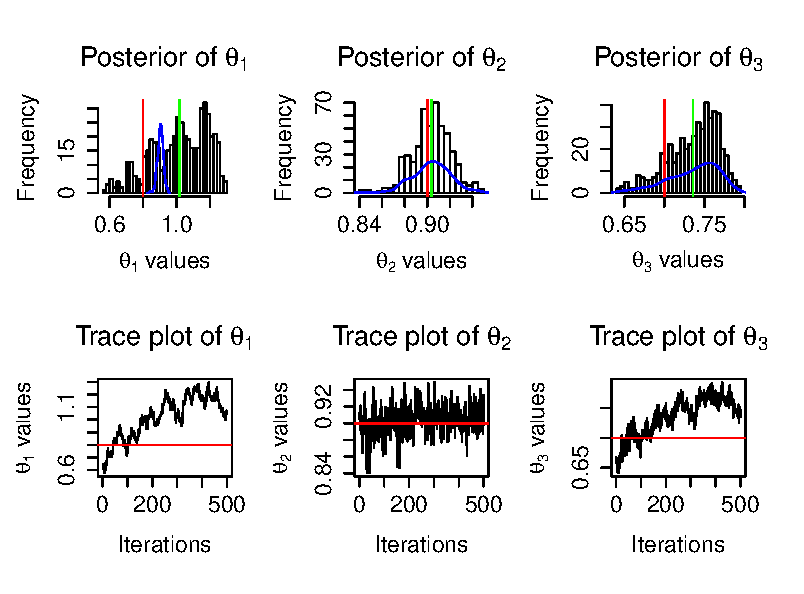
\includegraphics[width=140mm]{hmcplots7_combined.eps}
\caption{HMC plot 7 with positive $\theta_3$ and varying $\theta_1$}
\end{figure}

\lstinputlisting[float = h, frame = tb, caption = R output for plot 7 using the library CODA with varying $\theta_1$ and 20 steps of leapfrog with 0.001 $\epsilon$, label = hmcoutput7]{output7.txt}




% \begin{figure}[h]
% \centering
% 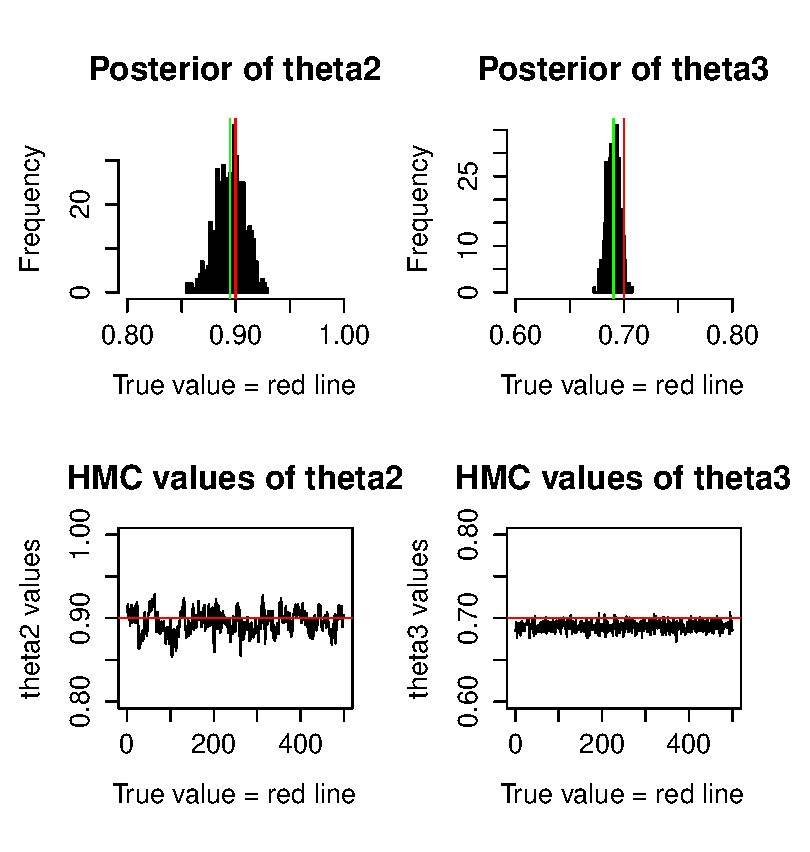
\includegraphics[width=100mm]{hmcplots8_modified3.eps}
% \caption{HMC plot 8 with constant $\theta_1 = 0.8$ and positive $\theta_3$ with 10 leapfrog steps}
% \end{figure}


% \begin{figure}[h]
% \centering
% 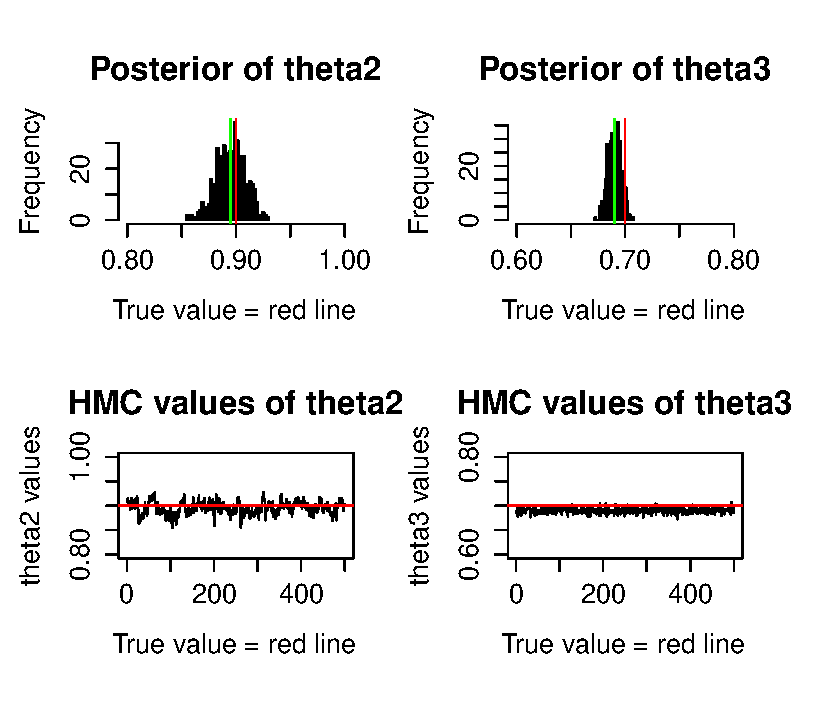
\includegraphics[width=150mm]{hmcplots9.eps}
% \caption{HMC plot 9 with constant $\theta_1 = 0.8$ and positive $\theta_3$ with 5 leapfrog steps}
% \end{figure}

\newpage
For better inference with HMC, we consider the first parameter to be a constant value of $\theta_1 = 0.8$

\begin{figure}[H]
\centering
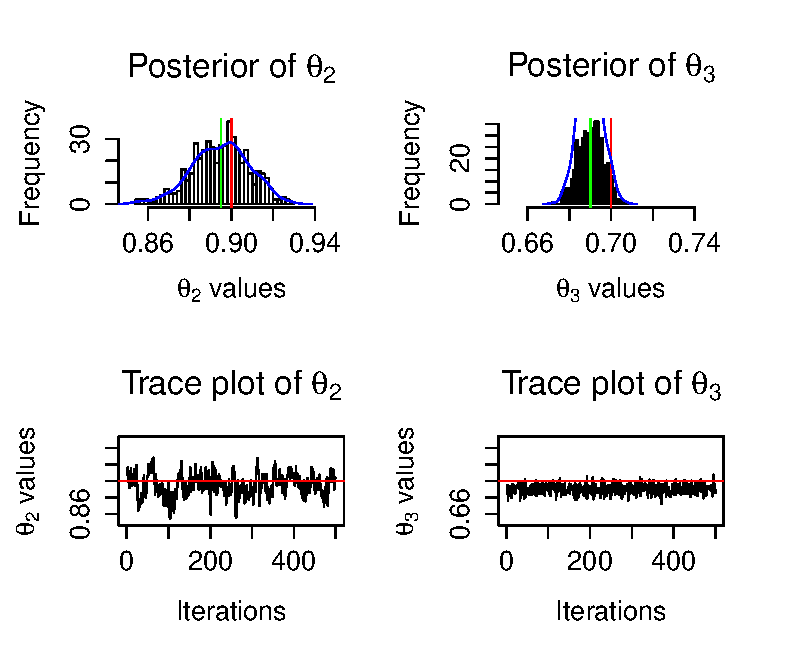
\includegraphics[width=150mm]{hmcplots8_combined.eps}
\caption{Trace plots, density and histograms for HMC 8 with constant $\theta_1 = 0.8$ and positive $\theta_3$ with 5 leapfrog steps}
\end{figure}

\lstinputlisting[float = h, frame = tb, caption = R output for plot 8 using the library CODA with 10 steps and 0.001 $\epsilon$, label = hmcoutput8]{output8.txt}

% \begin{figure}[H]
% \centering
% 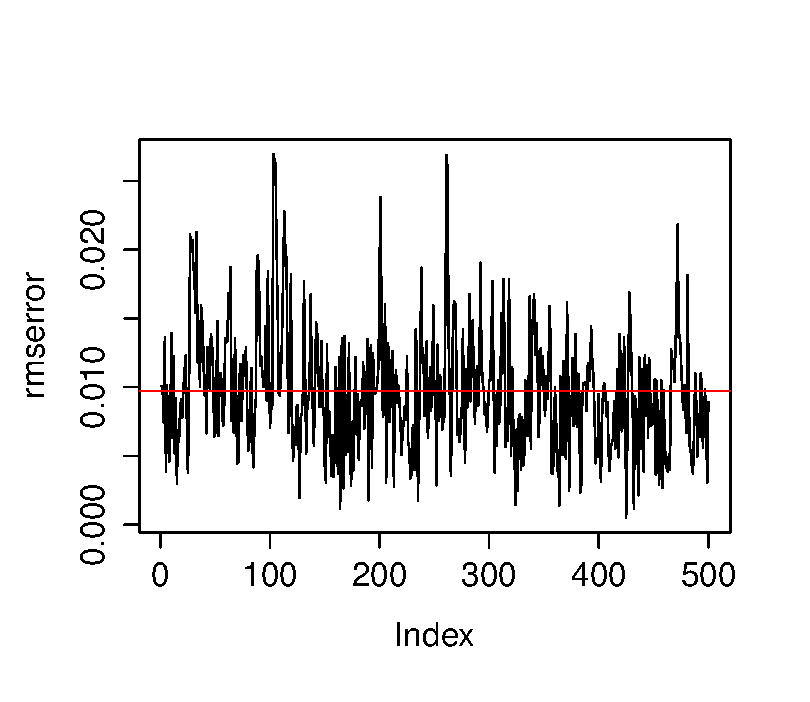
\includegraphics[width=100mm]{rmserror8.eps}
% \caption{Error plot after removing burnin period for HMC plot 8}
% \end{figure}

\begin{figure}[H]
\centering
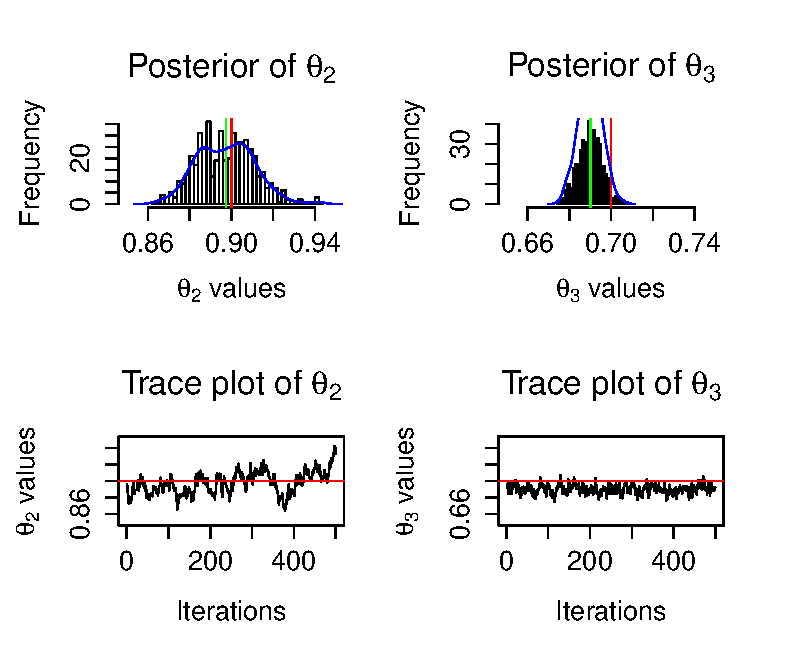
\includegraphics[width=150mm]{hmcplots9_combined.eps}
\caption{Trace plots, density and histograms for HMC 9 with constant $\theta_1 = 0.8$ and positive $\theta_3$ with 10 leapfrog steps}
\end{figure}

\lstinputlisting[float = h, frame = tb, caption = R output for plot 9 using the library CODA with 5 steps and 0.001 $\epsilon$, label = hmcoutput9]{output9.txt}

\begin{figure}[H]
\centering
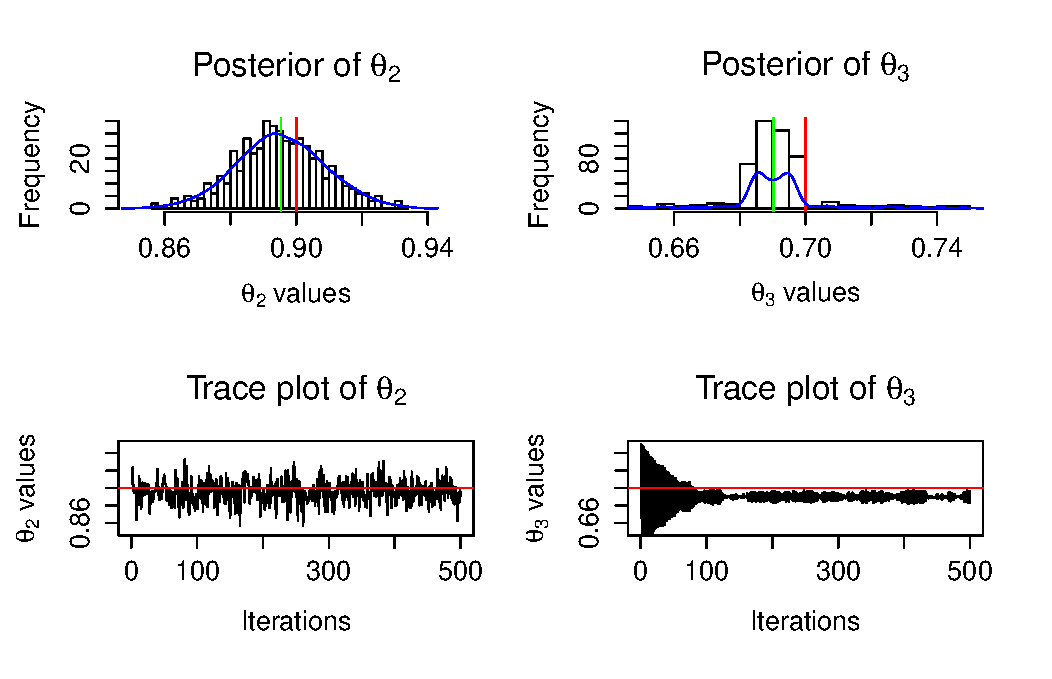
\includegraphics[width=150mm]{hmcplots10_combined.eps}
\caption{Trace plots, density and histograms for HMC 10 with constant $\theta_1 = 0.8$ and positive $\theta_3$ with 20 leapfrog steps and $\epsilon = 0.001$}
\end{figure}

\lstinputlisting[float = h, frame = tb, caption = R output for plot 10 using the library CODA with 20 steps and 0.001 $\epsilon$, label = hmcoutput8]{output10.txt}

\begin{figure}[H]
\centering
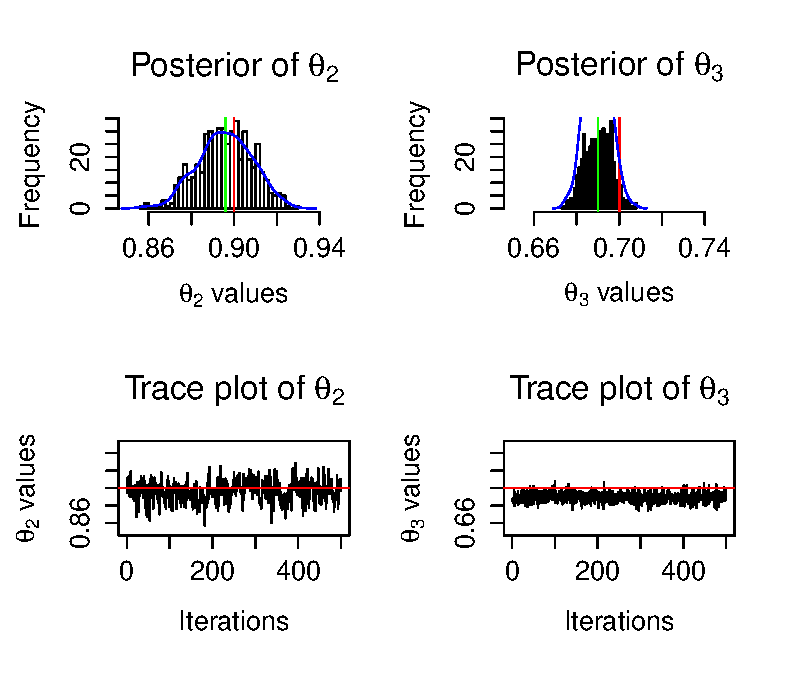
\includegraphics[width=150mm]{hmcplots11_combined.eps}
\caption{Trace plots, density and histograms for HMC 11 with constant $\theta_1 = 0.8$ and positive $\theta_3$ with 20 leapfrog steps}
\end{figure}

\lstinputlisting[float = h, frame = tb, caption = R output for plot 11 using the library CODA with 20 steps and 0.005 $\epsilon$, label = hmcoutput8]{output11.txt}

% \begin{figure}[H]
% \centering
% 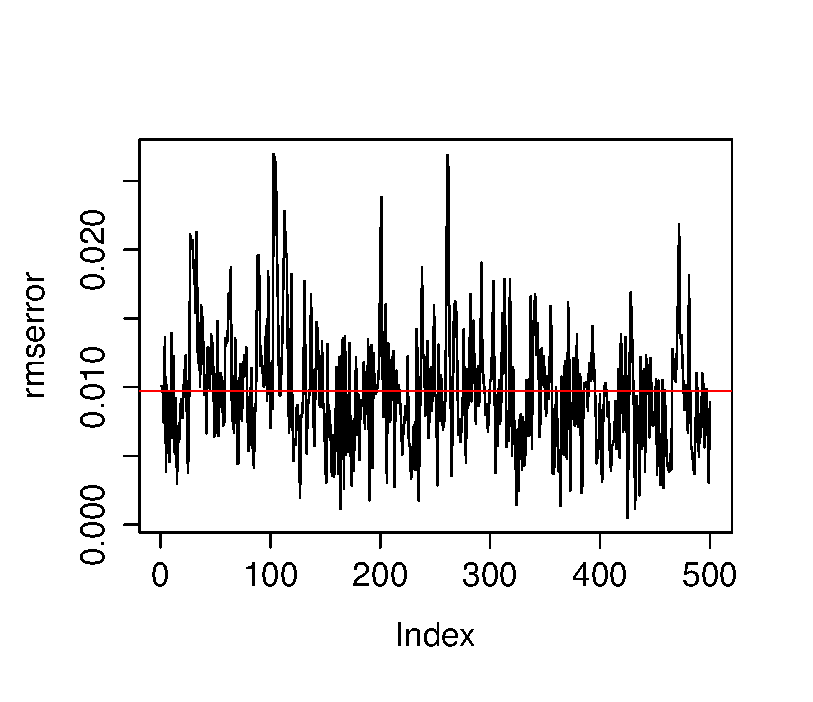
\includegraphics[width=50mm]{rmserror9.eps}
% \caption{Error plot after removing burnin period for HMC plot 9}
% \end{figure}


\begin{figure}[H]
    \centering
    \begin{subfigure}[b]{0.4\textwidth}
            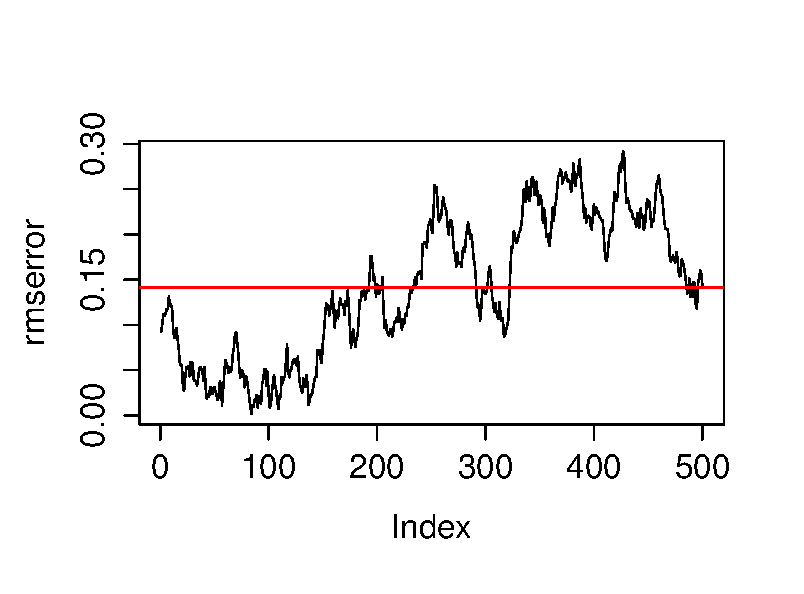
\includegraphics[width=\textwidth]{rmserror7.eps}
            \subcaption{HMC Plot 7}
    \end{subfigure}
    
    \begin{subfigure}[b]{0.4\textwidth}
            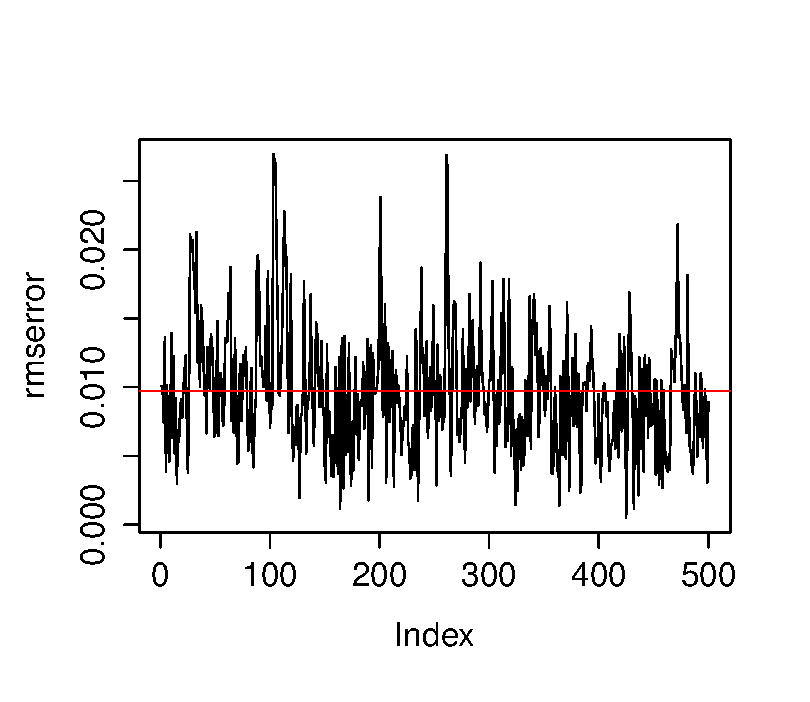
\includegraphics[width=\textwidth]{rmserror8.eps}
            \subcaption{HMC Plot 8}
    \end{subfigure}
    ~
    \begin{subfigure}[b]{0.4\textwidth}
            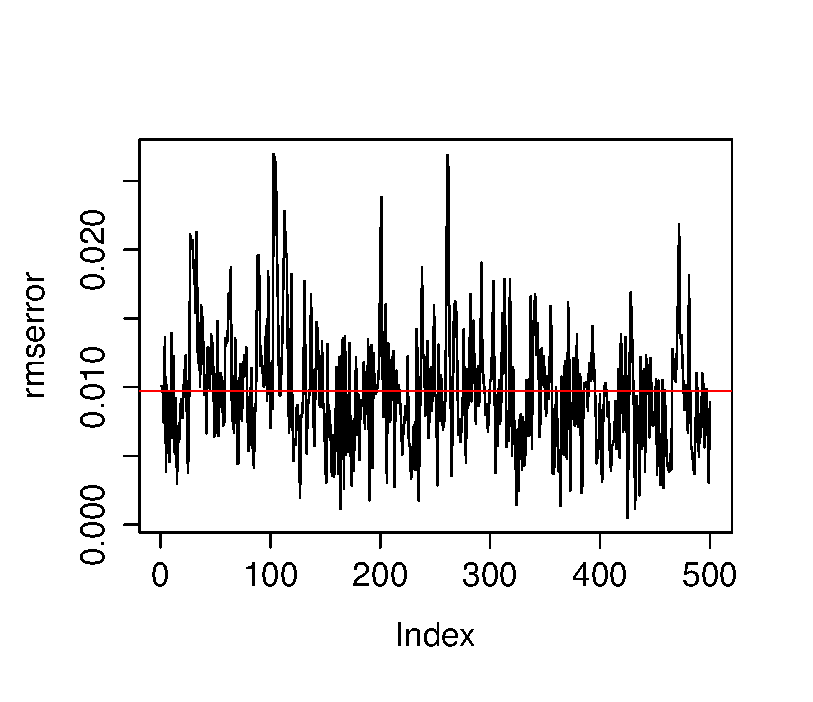
\includegraphics[width=\textwidth]{rmserror9.eps}
            \subcaption{HMC Plot 9}
    \end{subfigure}
    
    \begin{subfigure}[b]{0.4\textwidth}
            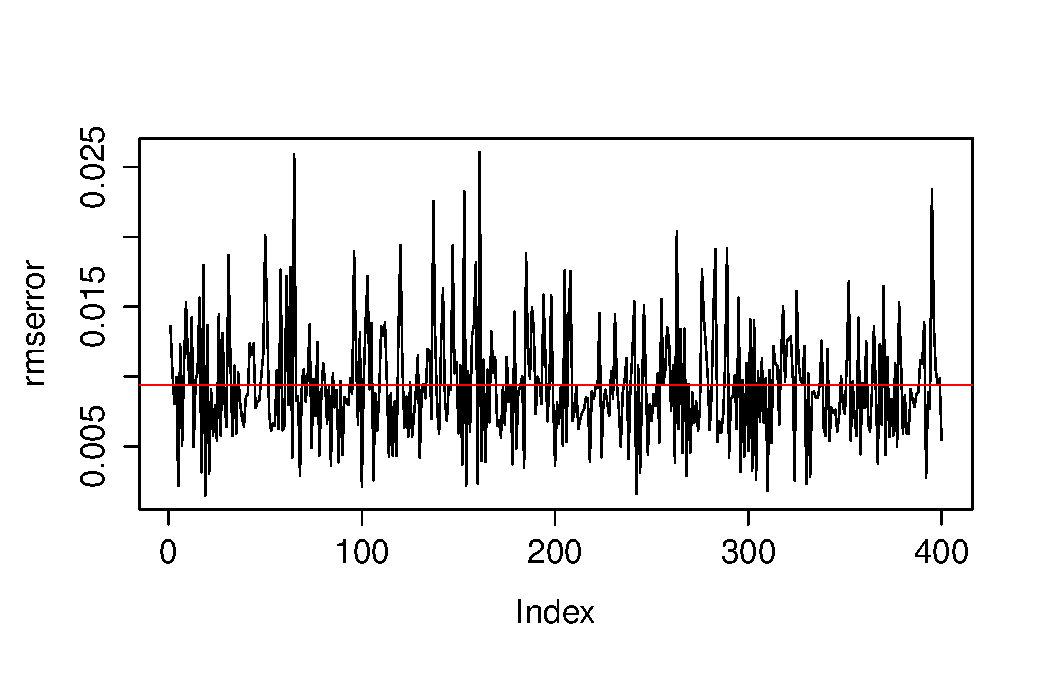
\includegraphics[width=\textwidth]{rmserror10.eps}
            \subcaption{HMC Plot 10}
    \end{subfigure}
    ~
    \begin{subfigure}[b]{0.4\textwidth}
            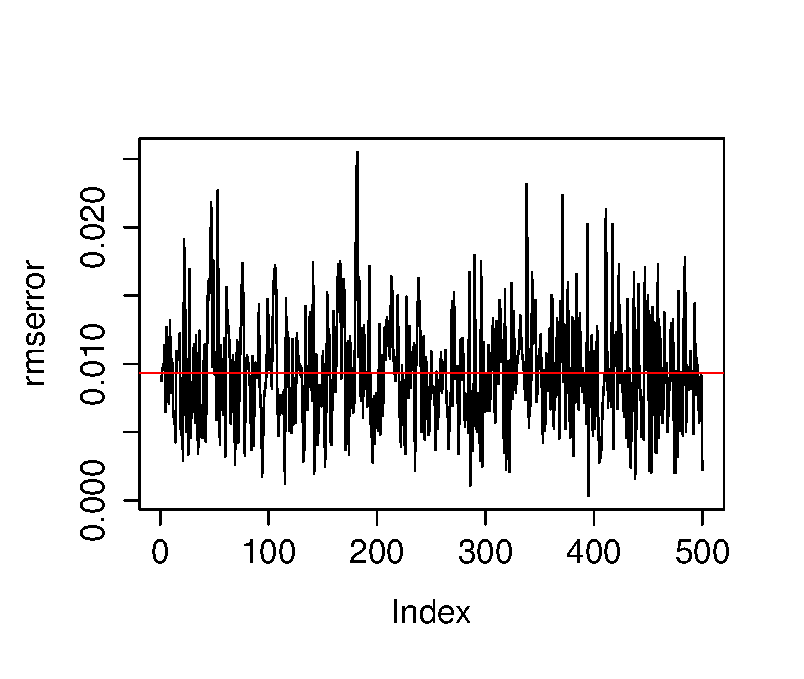
\includegraphics[width=\textwidth]{rmserror11.eps}
            \subcaption{HMC Plot 11}
    \end{subfigure}
    \caption{Error plot after removing burnin period for HMC plot} 
\end{figure}


\begin{figure}[h]
\centering
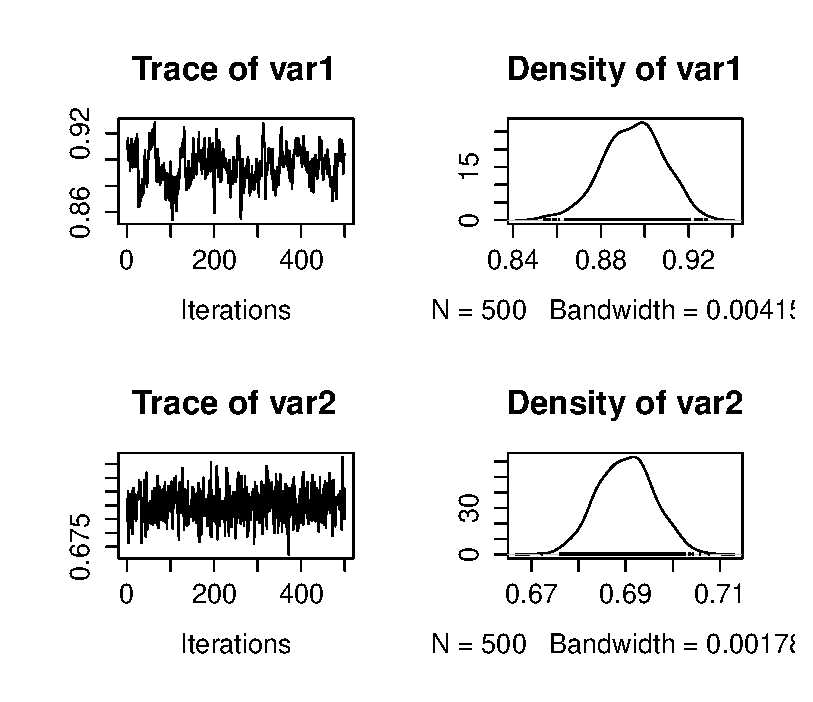
\includegraphics[width=140mm]{hmcplot_mcmc8.eps}
\caption{HMC plot 8 summary}
\end{figure}

\begin{figure}[h]
\centering
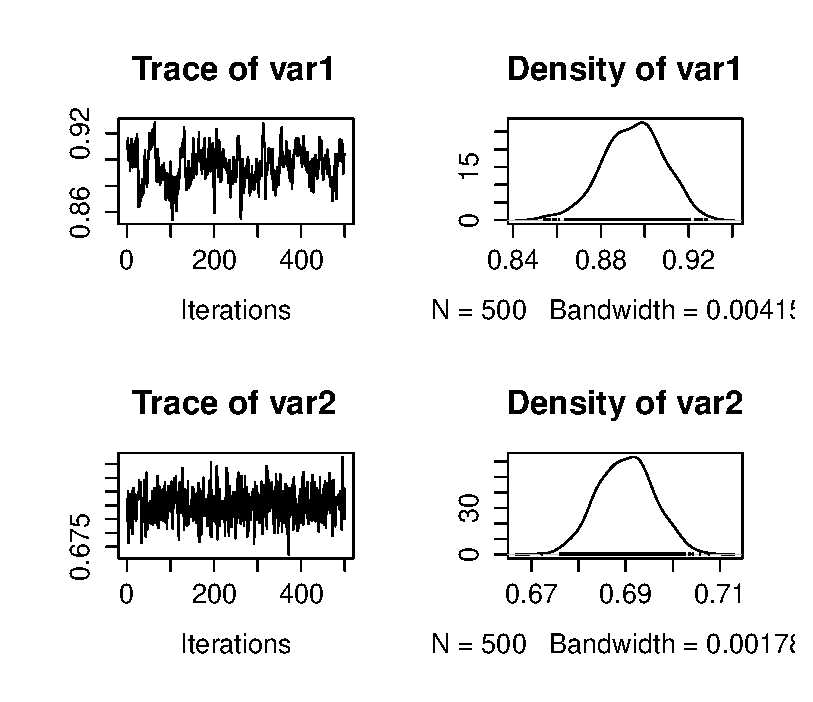
\includegraphics[width=140mm]{hmcplots9_mcmc.eps}
\caption{HMC plot 9 summary}
\end{figure}

\end{document}


